\chapter{Ý tưởng}
\label{ch:idea}

\section{Mixture of Experts: khái niệm cốt lõi}

Mixture of Experts (MoE)~\cite{jacobs1991adaptive,shazeer2017moe,mu2025survey} giải quyết bài toán bằng nhiều mạng chuyên biệt $E_1,\dots,E_n$ và một mạng nhỏ gọi là \emph{bộ định tuyến} (router) hay cổng, $G$, quyết định mỗi chuyên gia được tính bao nhiêu cho đầu vào hiện tại (Hình~\ref{fig:moe}):
\begin{equation}
\mathrm{MoE}(x)=C\big(\{G_i(x)\cdot E_i(x)\}_{i=1}^{n}\big),
\label{eq:moe}
\end{equation}
trong đó $G_i(x)$ là mức đóng góp của chuyên gia $i$ và $C$ là một hàm kết hợp, theo cách cổ điển là phép cộng. Vì $G$ nhận $x$ làm đầu vào, mức đóng góp thay đổi từ đầu vào này sang đầu vào khác. Đây chính là hành vi động mà mục tiêu O1 yêu cầu.

\begin{figure}[htbp]
  \centering
  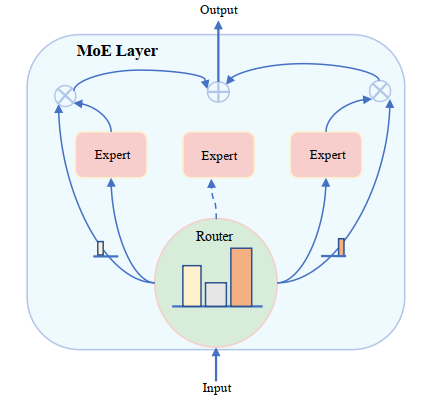
\includegraphics[width=.38\linewidth]{arch_moe.png}
  \caption{Một lớp Mixture of Experts, theo Mu và Lin~\cite{mu2025survey}. Bộ định tuyến đặt mức đóng góp của mỗi chuyên gia cho đầu vào hiện tại.}
  \label{fig:moe}
\end{figure}

\section{Từ kết hợp đầu ra đến kết hợp trọng số}

Phương trình~\eqref{eq:moe} kết hợp \emph{đầu ra} của các chuyên gia. Nếu áp dụng trực tiếp, mọi chuyên gia phải chạy cho mọi đầu vào, nên chi phí suy luận tăng theo số chuyên gia và các chuyên gia cần một không gian đầu ra chung. Weight-Ensembling Mixture of Experts (WEMoE)~\cite{tang2024wemoe} giữ bộ định tuyến nhưng thay đổi đối tượng được kết hợp. Mỗi chuyên gia được biểu diễn bằng véc-tơ tác vụ của nó, giá trị của bộ định tuyến nhân vào các véc-tơ đó, và trọng số kết quả được dựng lên trước khi áp dụng (Hình~\ref{fig:we}).

Hai cách này không tương đương. Với một lớp tuyến tính, $(\sum_i w_iW_i)h=\sum_i w_i(W_ih)$, nhưng đẳng thức này không còn đúng qua các hàm kích hoạt phi tuyến và các lớp xếp chồng. Do đó, kết hợp trọng số định nghĩa một hàm khác với tổ hợp đầu ra của các chuyên gia. Lợi ích tiềm năng của nó là một lượt truyền xuôi (forward pass) cho mỗi đầu vào, một checkpoint và một encoder dùng chung. Chi phí của nó là véc-tơ tác vụ phải được lưu cho mọi mô-đun nâng cấp, bộ định tuyến cần dữ liệu để huấn luyện, và mỗi đầu vào cần dựng trọng số riêng lúc chạy, điều này có thể làm suy luận chậm hơn ngay cả khi lưu ít tham số hơn. Mục~\ref{sec:efficiency} đo các chi phí này.

\begin{figure}[htbp]
  \centering
  \resizebox{.62\linewidth}{!}{\input{figures_vi/weight_ensembling}}
  \caption{Kết hợp ở mức tham số được dùng trong nghiên cứu này (a), đối chiếu với kết hợp ở mức đầu ra (b), chỉ được vẽ để tham khảo.}
  \label{fig:we}
\end{figure}

\section{Luồng thực hiện: từ dữ liệu đến đánh giá}
\label{sec:flow}

Hình~\ref{fig:flow} cho thấy luồng thực hiện gồm bốn chặng. Chặng 1 chuẩn bị năm tác vụ GLUE và chia mỗi tập huấn luyện chính thức thành ba phần. Chặng 2 tinh chỉnh một chuyên gia cho mỗi tác vụ từ mô hình huấn luyện trước, rồi giữ lại véc-tơ tác vụ và đầu phân loại (head) của nó. Chặng 3 hợp nhất chúng thành một mô hình và huấn luyện các bộ định tuyến trên tập few-shot. Chặng 4 báo cáo điểm trên các tập kiểm định chính thức, cùng dung lượng lưu trữ và độ trễ. Tập phát triển chọn epoch tốt nhất, hệ số tỉ lệ $\lambda$ và bước tốt nhất của bộ định tuyến, nên không lựa chọn nào chạm vào dữ liệu được báo cáo. Trọng số chuyên gia được đóng băng sau Chặng 2, và chỉ các bộ định tuyến học ở Chặng 3.

\begin{figure}[htbp]
  \centering
  \resizebox{.8\linewidth}{!}{\input{figures_v3_vi/flow}}
  \caption{Luồng thực hiện: từ dữ liệu đến đánh giá. Mũi tên nét đứt cho biết nơi tập phát triển chọn mô hình. $\theta_i$ và $\tau_i$ được định nghĩa ở Mục~\ref{sec:problem}, $g_i$ là head của chuyên gia $i$, và $\lambda$ là hệ số tỉ lệ của Task Arithmetic ở Mục~\ref{sec:ta}.}
  \label{fig:flow}
\end{figure}
